\chapter{Analysis}

Here we will look at the performance profile of our various configurations.
Note that we are running everything on a software network simulator, and
therefore these performance tests will only be useful for giving us an
indication of \textit{relative} performances.

Therefore we will first need to establish a baseline for the system as it
is. We should then be able to compare various configurations against it.

\todo{Når ferdig, test med ekte software som MySQL, osv osv.}

For reference, the teste have been run on an Ubuntu GNU/Linux VM from the
Mininet site, loaded with our code and running in VirtualBox on a Mac OS X
laptop.

Instructions on how to run the tests are given in
\ref{chapter:appendix.benchmark}
\vpageref{chapter:appendix.benchmark}.

\section{Baseline --- ICMP ping on L2 learning switch using flow tables}
\label{chapter:baseline.benchmark}

The most basic setup we can test against is using our L2 learning switch
from chapter \ref{chapter:l2.learning.switch}
\vpageref{chapter:l2.learning.switch}.  This is fundamental to all our
configurations, because they all use it to make sure that packets are routed
correctly.

We will use the topology given in figure \ref{figure:baseline.topology}.

\begin{figure}
  \centering
  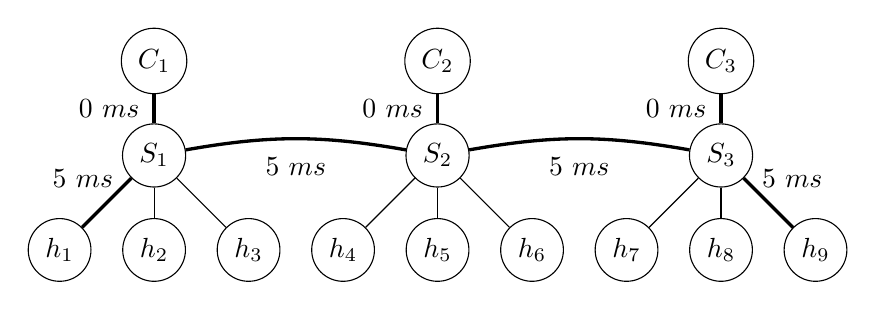
\begin{tikzpicture}[
    every node/.style={draw, circle},
    x=0.6cm,
    y=0.6cm]

    % Switches
    \foreach \n in {1,2,3} {
      \pgfmathsetmacro\x{(\n-2)*6}

      % Switch
      \node (S\n) at (\x ,  0) {$S_\n$};

      % Controller
      \node (C\n) at (\x ,  2) {$C_\n$};
      \draw (S\n) -- (C\n);

      % Hosts
      \foreach \h in {1,2,3} {
        \pgfmathsetmacro\pos{(\h - 2)*2}
        \pgfmathtruncatemacro\num{((\n - 1)*3) + int(\h)}

        % Host node
        \node (h\num) at (\x + \pos, -2) {$h_{\num}$};
        \draw (S\n) -- (h\num);
      }
    }

    % Switch links
    \draw (S1) to[out=10,in=170]
               node[below=-0.2cm, draw=none] {$5~ms$} (S2);

    \draw (S2) to[out=10,in=170]
               node[below=-0.2cm, draw=none] {$5~ms$} (S3);

    % Mark traversal path
    \draw [very thick] (h1) -- node[above left=-0.1cm,draw=none] {$5~ms$} (S1);
    \draw [very thick] (S1) -- node[left,draw=none] {$0~ms$} (C1);
    \draw [very thick] (S1) to[out=10,in=170] (S2);

    \draw [very thick] (S2) -- node[left,draw=none] {$0~ms$} (C2);
    \draw [very thick] (S2) to[out=10,in=170] (S3);

    \draw [very thick] (S3) -- node[left,draw=none] {$0~ms$} (C3);
    \draw [very thick] (S3) -- node[above right=-0.1cm,draw=none] {$5~ms$} (h9);
  \end{tikzpicture}
  \caption{Baseline topology with three switches $S$ and their controllers
    $C$.  The client $c_0$ will send ICMP ping packets to the farthest node
      $h_9$.  The packets will go through three links with a configured
      latency of $5~ms$.}
  \label{figure:baseline.topology}
\end{figure}

Before we present the results, let's look at what we should expect from the
configuration above.  The three links the packets need to cross each have
$5~ms$ latency.  There is some latency in each switch and in each end of the
link ($c_0$ and $h_9$) as well as between and in the switches and their
controllers.

In total, one would expect the \acf{RTT} to be
\begin{gather}
  RTT_{c_0, h_9} = 2\left( \sum L + \sum P_S + \sum P_C \right) + P_{c_0} + P_{h_9} + K
  \label{equation:baseline.rtt}
\end{gather}

That is, the one--way latencies for all links ($L_{h_1,S_1}$, etc.), processing time $P$ for
$S,~C,~c_0,~h_9$ and a constant $K$ for any extra noise on the network
(e.g., from the OS, virtual machine engine, when flushing file buffers for
 recording results and so on).
Equation \ref{equation:baseline.rtt} is inspired by \cite{DBLP:conf/cnsm/PhemiusB13}.
\todo{Refiner formel, den kan ha feil!}

For simplicity, we will set $P_{c_0},~P_{h_9}$ and the
latencies for links between switches and controllers to zero.\footnote{When
flow table entries are installed, one should see very little traffic going
to the controllers, meaning that we can
assume that $L_{C,S} \to 0$ when the flow tables have been ramped up.
There will still be some background noise on the network, though, and we
print the ones we don't have rules for as dots in the controller log.}
We have also removed the fall--back link
between $S_1$ and $S_3$ seen in figure \ref{figure:graph.three.switches}
to make sure that ICMP packets won't take different paths on the network.
We could attempt to measure $K$ by running Mininet with two nodes linked
with zero bandwidth, but we will simply set it to zero as well.

Filling in the known values gives
\begin{gather}
  RTT_{c_0,h_9} = 40~ms + 2\left( \sum P_S + \sum P_C \right)
  \\
  RTT_{c_0,h_9} = 40~ms + 2L~\text{where}~L = \sum P_S + \sum P_C
  \label{equation:expected.baseline.rtt}
\end{gather}

We will now use the \texttt{ping} command to send out many packets per
second.  The controller will install flow tables with idle and hard timeout
set to one hour. The flows we install (flow table entries) will match on
Ethernet packets whose destination addresses are on known ports.

Table \ref{table:baseline.summary} gives a summary and figure
\ref{benchmark:l2.learning.switch.ping} shows the plots.

% Table with summary of RTTs (mean, median, etc.)
\input{data/pings-summary.tex}

\begin{figure}
  \centering
  \includegraphics[width=\textwidth]{data/pings.pdf}
  \caption{\acs{RTT} for ICMP PING on the L2 learning switch using flow tables.
           We can clearly see the ramp--up time for the controller as it
           adds flow table entries to have the switch automatically forward
           Ethernet packets. The plot shows the \textit{median} value in red
  and the \textit{mean} in gray.  Because of the ramp--up phase, the mean is a poor
  indicator for the values after warm--up.  As we have a relatively large
  number of samples, the median gives a more realistic picture of the
  situation.  This can clearly be seen in the plot.}
  \label{benchmark:l2.learning.switch.ping}
\end{figure}

There is a noticeable ramp--up time before flow tables get entries, and
because of this we will have some variation in the samples. Therefore we
would assume to get a mean value larger than the median.  Looking at the
histogram, this seem to be the case, and therefore the median should give a
more realistic value for the RTT when the system has settled down.

Other than that, we see that the median is in line with our
expectations---the RTT is clearly bound an RTT of 40 ms.  We can now insert
the median value in equation \ref{equation:expected.baseline.rtt}.

\input{data/pings-results.tex}

If we run the test again \textit{without} installing flows, we should see
all the processing being moved over to the controllers.  This should let us
give an estimate for $P_C$.

We ran the test again  with the only difference being that we don't
install flows.  The summary can be found in table
\ref{table:baseline.noflows.summary} and the plots in figure
\ref{figure:baseline.noflows.plots}.

Using the estimated value for $P_C$, we see that

\begin{gather*}
  L = 3P_S + \sum P_C = 1.60~ms \\
  \sum P_C = 3P_C = \frac{75.80~ms - 40~ms}{2} = 17.90~ms \\
  P_C \approx 5.97~ms
\end{gather*}
\todo{Put this part in an R script}

When all the work is being done by the controllers, their individual
one--way processing latency is around $5.97~ms$.  The ramp--up this time
refers to the fact that the controllers still need to populate their
MAC--to--port tables so they can forward packets instead of broadcasting
them.  There is also a spike in RTT at the very end.  We haven't looked more
into this.
\todo{Er en spike imot slutten også, hvorfor? Er det buffer-skriving?
  Isåfall, da burde den også være på forrige graf... hva skjer?
Og hvorfor er det så konsistent?}

\input{data/pings-noflows-summary.tex}

\begin{figure}
  \centering
  \includegraphics[width=\textwidth]{data/pings-noflows.pdf}
  \caption{Rerun of baseline benchmark
    (ch.~\ref{chapter:baseline.benchmark}), but without installing flows.}
  \label{figure:baseline.noflows.plots}
\end{figure}

\todo{Remove outliers and show numbers.}
\todo{Bruk boxplot() i R når en skal sammenligne. Og hiv inn tall i tabell
  for sammenligning sammen med plot. Plot trenger ikke være gigantisk stor.}

\section{L2 learning switch, key--value store}
\label{chapter:benchmark.l2.kv.noflows}

First we need a baseline.  Here we have a topology of two switches $S_0$ and
$S_1$ with a controller each.  The switches has three hosts, $h_0, \dots, h_5$.
A client $c_0$ is connected to $S_0$. We're running Python
key--value--stores on each host, and $c_0$ will issue a get--request
followed by a put--request to the host $h_5$, which is connected to $S_1$.
We measure the time for each request, divide it
by two and call it latency.\footnote{We basically assume that the packets
take an equal amount of time back and forth, and divide by two to get this
time.}

There are two controllers $C_0$ and $C_1$ for the switches $S_0$ and $S_1$,
respectively.  In this situation, the packets from $c_0$ need to travel
over two switches.

The network is running on Mininet, a software network simulator, on a Linux
virtual machine running on an Mac OS X box.  All the links in Mininet have
been set up with $10 Mbit/s$ bandwidth, $5~ms$ latency and no packet
loss.  These links have been set up with \ac{HTB}
\cite{devera2002hierarchical} enabled, which Open vSwitch\index{Open vSwitch}
 uses for providing rate limiting.

In this first benchmark, the switches will send each packet up to the
controllers.  The controllers implement L2 learning switches and will not
install any flow table entries for rapid dispatch.

On the x--axis is the time in seconds.  On the y--axis is the latency for
get and put requests.

The result can be seen in figure \ref{benchmark:l2.learning.switch.no.flows} 
\vpageref{benchmark:l2.learning.switch.no.flows}.

What is surprising here is that the put--requests have much higher latency
than the get--requests. We don't know why this is.\todo{Finn ut! Er det pga
  pakkene er større? Eller andre grunner?}

\section{L2 learning switch, key--value store, flow entries}

We have the same setup as above, but this time we install flow entries that
will automatically forward the packets.  The flow table entries will match
on as many fields in the packets as possible.

The flow table entries have idle and hard timeouts set to 10 seconds.
In other words, we should be able to see some increased latency every ten
seconds.

% Present both plots together
\begin{figure}
  \centering
  \begin{subfigure}{\textwidth}
    \centering
    \includegraphics[width=\textwidth]{data/data2.eps}
    \caption{L2 learning switch without using flow tables.}
    \label{benchmark:l2.learning.switch.no.flows}
  \end{subfigure}

  \centering
  \begin{subfigure}{\textwidth}
    \centering
    \includegraphics[width=\textwidth]{data/data3.eps}
    \caption{L2 learning switch using flow tables.}
    \label{benchmark:l2.learning.switch.with.flows}
  \end{subfigure}
\end{figure}

The result can be seen in figure \ref{benchmark:l2.learning.switch.with.flows}
\vpageref{benchmark:l2.learning.switch.with.flows}.

Here we can see that the latency has been reduced somewhat.\todo{Hvor mye?
Hva med å plotte over hverandre, hva med å lage average eller root mean
square eller noe sånn?}

We also see some latency spikes around every ten seconds, as expected.

\todo{Plott med flere verdier, istedenfor å vise seconds på x--aksen kan vi
  vise elapsed time, som i at den starter på 0 sekunder.}

These two benchmarks will serve as a baseline to which we will compare our
performance when we enable Paxos on the switches.

Remember that when we run Paxos, we will still have to use the L2 learning
switch for the nodes to be able to communicate.

\todo{Trendlinjner, moving average, fitting osv... må ha det i grafene, må
  også ha litt statistisk analyse av tallene selv osv.}

\section{Three switches, Paxos on controller}

\todo{Få data}

\section{Three switches, Paxos on controller and flow table}

\todo{Få data}

\section{Other solutions}

We chose to use OpenFlow as the basis for our system.
We could just as well have used a networking system that already supported
programmability in some way, for instance the Intel DPDK\todo{Needs
citation}.\todo{Also needs defense.}

\todo{Flytt evt dette ned til improvements--delen}
